\renewcommand{\theequation}{\theenumi}
\begin{enumerate}[label=\arabic*.,ref=\thesubsection.\theenumi]
\numberwithin{equation}{enumi}
%\item Find the remainder when $x^3+3x^2+3x+1$ is divided by 
%\begin{enumerate}
%\item $x+1$
%\item $x-\frac{1}{2}$
%\item $x$
%\item $x+\pi$
%\item $5+2x$
%\end{enumerate}
%%
%\item Check whether $7+3x$ is a factor of $3x^3+7x$.
%%
%\item Determine which of the following polynomials has $(x+1)$ as a factor:
%%
%\begin{enumerate}
%\item $x^3+x^2+x+1$
%\item $x^4+x^3+x^2+x+1$
%\item $x^4+3x^3+3x^2+x+1$
%\item $x^3-x^2-\brak{2+\sqrt{2}}+\sqrt{2}$.
%\end{enumerate}
%%
%\item Determine whether $g(x)$ is a factor of $p(x)$ in each of the following cases:
%%
%\begin{enumerate}
%\item $p(x) = 2x^3+x^2-2x-1, g(x) = x+1$
%\item $p(x) = x^3+3x^2+3x+1, g(x) = x+2$
%\item $p(x) = x^4-4x^2+x+6, g(x) = x-3$
%\end{enumerate}
%%
%\item  Factorise : 
%\begin{enumerate}
%\item $x^3 – 2x^2 – x + 2 $
%\item $x^3– 3x^2 – 9x – 5 $
% \item $x^3+ 13x^2 + 32x + 20 $
%\item $2y^3+ y^2– 2y – 1$
%\end{enumerate}
%\item Find the roots of the following equations:
%\begin{enumerate}
%\item  $x - \frac{1}{x} = 3, x \ne =0 $
%\item  $ \frac{1}{x+4} - \frac{1}{x-7} = \frac{11}{30}, x\ne =-4, 7 $
%\end{enumerate}
%%
%\item Find the slope of the tangent to the curve $y = 3x^4-4x$ at $x=4$.
%\item Find the slope of the tangent to curve $y = x^3-3x+2$ at the point whose 
%x-coordinate is 2.
%\item Find the slope of the tangent to the curve $y = x^3-3x+2 $ at the point whose x-coordinate is 3.
%\item Find the slope of the normal to the curve 
%$
%\vec{x} = a \myvec{\cos^3\theta \\ \sin^{3}\theta}
%$
%at $\theta = \frac{\pi}{4}$.
%\item Find the slope of the normal to the curve 
%$
%\vec{x} =  \myvec{1-a\sin\theta \\ b\cos^{2}\theta}
%$
%at $\theta = \frac{\pi}{2}$.
%\item Find points at which the tangent to the curve $y = x^3-3x^2-9x+7$ is parallel to th x-axis.
%\item Find the point on the curve $y = x^3– 11x + 5$
%at which the tangent is $\myvec{1 & -1}\vec{x} =  11$.
%\item Find the equations of all lines having slope 0 which are tangent to the curve 
%$
%y = \frac{1}{x^2-2x+3}
%$.
%\item Find the equations of the tangent and normal to the given curves at the indicated points: 
%%
%\begin{enumerate}
%\item
%$
%y= x^4 - 6x^3+13x^2-10x+5
%$
%at \myvec{0\\5}.
%\item
%$
%y = x^4 - 6x^3+13x^2-10x+5
%$
%at \myvec{1\\3}.
%\item
%$
%y = x^3
%$
%at \myvec{1\\1}.
%\end{enumerate}
%%
%\item Show that the tangents to the curve $y = 7x^3 + 11$ at the points where $x = 2$ and $x = -2$ are parallel.
%\item Find the points on the curve $y = x^3$  at which the slope of the tangent is equal to the y-coordinate of the point.
%\item For the curve $y = 4x^3 – 2x^5$ find all the points at which the tangent passes through the origin.
%\item Find the equation of the normal at the point $\myvec{am^2 \\ am^3}$  for the curve $ay^2 = x^3$
%\item Find the equation of the normals to the curve $y = x^3+2x+6$ which are parallel to the line $\myvec{1 & 14} + 4 = 0$.
%\item Find the slope of the normal to the curve $y = 2x^2 + 3 \sin x$ at $x = 0$.
%%
%Show that the normal at any point $\theta$ to the curve $\vec{x} = \myvec{a \cos\theta + a \theta \sin\theta\\  a \sin\theta – a\theta \cos\theta}$ is at a constant distance from the origin.
%%
%\item Find the slope of the tangent to the curve $\vec{x} = \myvec{t^2+3t-8 \\ 2t^2-2t-5}$
%at the point $\myvec{2\\-1}$.
%\item Find the points on the curve $9y^2 = x^3$, where the normal to the curve makes equal intercepts with the axes.
%\item Find the area under $y = x^4, x = 1, x = 5$ and x-axis.
%%
%\item Find the area bounded by the curve $y = x^3, x =-2, x = 1$ and the x-axis.
%\item Find the area bounded by the curve $y = x \abs{x}, x = -1, x = 1$ and the x-axis.
%\item Find the area bounded by the y-axis, $y = \cos x$ and $y = \sin x$ when $0 \le x \le \frac{\pi}{2}$.\item Show that the function given by $f(x) = 3x+17$  is increasing on $\vec{R}$.
%\item Show that the function given by $f(x) = e^{2x}$  is increasing on $\vec{R}$.
%%
%%
%\item Show that the function given by 
%\begin{align}
%f(x)  = \sin x
%\end{align}
%%
%is 
%\begin{enumerate}
%\item increasing in $\brak{0,\frac{\pi}{2}}$
%\item decreasing in $\brak{\frac{\pi}{2}, \pi}$
%\end{enumerate}
%%
%%
%\item Find the intervals in which the function given by 
%\begin{align}
%f(x)  = 2x^3-3x^2 - 36x +7
%\end{align}
%%
%is 
%\begin{enumerate}
%\item increasing
%\item decreasing.
%\end{enumerate}
%%
%\item Find the intervals in which the following functions are strictly increasing or decreasing
%%
%\begin{enumerate}
%\item $\brak{x+1}^3\brak{x-3}^3$
%\item $-2x^3-9x^2-12x+1$
%\end{enumerate}
%%
%\item Show that 
%%
%\begin{align}
%y = \log \brak{1+x}-\frac{2x}{2+x}, x > -1,
%\end{align}
%%
%is an increasing function of $x$ throughout its domain.
%%
%\item Find the values of $x$ for which $y = x\brak{x-2}^2$ is an increasing function.
%%
%\item Prove that
%%
%\begin{align}
%y = \frac{4\sin \theta}{2+\cos \theta} - \theta
%\end{align}
%%
%is an incresing function of $\theta$ in $\sbrak{0,\frac{\pi}{2}}$.
%\item Prove that the logarithmic function is increasing on $\brak{0, \infty}$.
%\item Which of the following functions are decreasing on $\sbrak{0,\frac{\pi}{2}}$?
%%
%\begin{enumerate}
%\item $\cos x$
%\item $\cos 2x$
%\item $\cos 3x$
%\item $\tan x$
%\end{enumerate}
%%
%\item Find the intervals on which 
%%
%\begin{align}
%f(x) = x^{100}+\sin x -1
%\end{align}
%%
%is decreasing.
%\item Let $I$ be any interval disjoint from $\sbrak{1,-1}$.  Prove that the function $f$ given by $f(x) = x +\frac{1}{x}$ is increasing on $I$.
%\item Prove that the function $f$ given by $f(x) = \log \sin x$ is increasing on $\brak{0,\frac{\pi}{2}}$ and decreasing on $\brak{\frac{\pi}{2}, \pi}$.
%\item Prove that the function $f$ given by $f(x) = \log \abs{\cos x}$ is decreasing on $\brak{0,\frac{\pi}{2}}$ and increasing on $\brak{\frac{3\pi}{2}, 2\pi}$.
%\item Prove that the function given by $f(x) = x^3-3x^2+3x-100$ is increasing in $\vec{R}$.
%\item Find the interval(s) in which $f(x) = x^2e^{-x}$ is increasing.
%\item Find the maximum and minimum values, if any, of $g(x) = x^3+1$.
%%
%\item Find the maximum and minimum values, if any of
%the following functions given by 
%%
%\begin{enumerate}
%\item $h(x) = \sin\brak{2x} + 5$
%\item $f(x) = \abs{\sin\brak{4x} + 3}$
%\end{enumerate}
%%
%\item Find the local maximum and minima, if any, of
%the following functions.  Find also the  local maximum and local minimum values, as the case may be
%%
%\begin{enumerate}
%\item $g(x) = x^3-3x$
%\item $h(x) = \sin x +\cos x, x \in \brak{0,\frac{\pi}{2}}$
%\item $f(x) = \sin x -\cos x, x \in \brak{0,2\pi}$
%\item $f(x) = x^3-6x^2+9x+15$
%\item $g(x) = \frac{x}{2} + \frac{2}{x}, x > 0$
%\item $g(x) = \frac{1}{x^2+2}$
%\item $f(x) = x\sqrt{1-x}, 0 < x < 1$.
%\end{enumerate}
%%
%\item Prove that the following functions do not have maxima or minima:
%%
%\begin{enumerate}
%\item $f(x) = e^x$
%\item $g(x) = \log x$
%\item $h(x) = x^3+x^2+x+1$
%\end{enumerate}
%\item Find the absolute maximum and absoute minimum value of the following functions in the given intervals
%%
%\begin{enumerate}
%\item $f(x) = x^3, x \in \brak{-2,2}$
%\item $f(x) = \sin x + \cos x,  x \in \brak{0,\pi}$.
%\end{enumerate}
%%
%\item Find both the maximum value and the minimum value of 
%\begin{align}
%3x^4-8x^3+12x^2-48x+25, x \in \sbrak{0,3}.
%\end{align}
%%
%\item At what points in the interval $\sbrak{0,2\pi}$, does the function $\sin 2x$ attain its maximum value?
%\item What is the maximum value of the function $\sin x + \cos x$?
%\item Find the maximum value of $2x^3-24x+107$ in the interval $\sbrak{1,3}$.  Find the maximum value of the same function in $\sbrak{-3,1}$.
%\item It is given that at $x=1$, the function $x^4-62x^2 + ax+9$ attains its maximum value on the interval $\sbrak{0,2}$.  Find the value of $a$.
%\item Find the maximum and minimum values of $x + \sin 2x$ on $\sbrak{0, 2\pi}$.
%\item For all real values of x, the minimum value of
%\begin{align}
%\frac{1-x+x^2}{1+x+x^2}.
%\end{align}
%%
%\item Find the maximum value of 
%\begin{align}
%\sbrak{x\brak{x-1}}^{\frac{1}{3}}.
%\end{align}
%\item Using differentials, find the approximate value of each of the following
%%
%\begin{enumerate}
%\item $\brak{\frac{17}{81}}^{\frac{1}{4}}$
%\item $\brak{33}^{-\frac{1}{5}}$
%\end{enumerate}
%%
%\item Show that the function given by $f(x) = \frac{\log x}{x}$ has maximum at $x = 3$.
%\item Find the intervals in which the function $f$ given by 
%%
%\begin{align}
%f(x)  = \frac{4\sin x-2x - x\cos x}{2+\cos x}
%\end{align}
%%
%is
%%
%\begin{enumerate}
%\item increasing 
%\item decreasing 
%\end{enumerate}
%%
%\item Find the interals in which the function $f$ given by 
%%
%\begin{align}
%f(x)  = x^3 + \frac{1}{x^3}, \quad x \ne 0
%\end{align}
%%
%is
%\begin{enumerate}
%\item increasing 
%\item decreasing 
%\end{enumerate}
%%
%\item Find the absolute maximum and minimum values of the function $f$ given by 
%%
%\begin{align}
%f(x)  = \cos^2 x + \sin x , \quad x \in \sbrak{0,\pi}
%\end{align}
%%
%\item Find the points at which the function $f$ given by 
%%
%\begin{align}
%f(x)  = \brak{x-2}^4\brak{x+1}^3
%\end{align}
%%
%has
%\begin{enumerate}
%\item local maxima
%\item local minima
%\item point of inflexion
%\end{enumerate}
%%
%\item Examine the following functions for continuity.
%%
%\begin{enumerate}
%\item $f(x) = \frac{1}{x-5}$
%\item $f(x) = \frac{x^2-25}{x+5}, x \ne -5$
%\end{enumerate}
%%
%\item Prove that the function $f(x) = x^n$ is continuous at $x = n$, where $n$ is a positive integer.
%%
%\begin{enumerate}
%\item 
%$
%\begin{alignedat}[t]{2}
%f(x)=
%\begin{cases}
%x^3-3, & x \le 2,
%\\
%x^2+1, & x > 2
%\end{cases}
%\end{alignedat}
%$
%\item 
%$
%\begin{alignedat}[t]{2}
%f(x)=
%\begin{cases}
%x^10-1, & x \le 1,
%\\
%x^2, & x > 1
%\end{cases}
%\end{alignedat}
%$
%\end{enumerate}
%%
%\item Discuss the continuity of the following functions:
%%
%\begin{enumerate}
%\item 
%$
%\begin{alignedat}[t]{2}
%f(x)= \sin x + \cos x
%\end{alignedat}
%$
%\item 
%$
%\begin{alignedat}[t]{2}
%f(x)= \sin x - \cos x
%\end{alignedat}
%$
%\item 
%$
%\begin{alignedat}[t]{2}
%f(x)= \sin x \cos x
%\end{alignedat}
%$
%\end{enumerate}
%\item Discuss the continuity of the cosine, cosecant, secant and cotangent functions.
%\item Find all points of discontinuity of $f$, where 
%\begin{align}
%f(x)=
%\begin{cases}
%\frac{\sin x}{x}, & x < 0,
%\\
%x+1, & x \ge 0
%\end{cases}
%\end{align}
%\item Determine if 
%\begin{align}
%f(x)=
%\begin{cases}
%x^2\sin \brak{\frac{1}{x}}, & x \ne 0,
%\\
%0, & x = 0
%\end{cases}
%\end{align}
%%
%is a continuous function.
%\item Examine the continuity of 
%\begin{align}
%f(x)=
%\begin{cases}
%\sin x -\cos x, & x \ne 0,
%\\
%-1, & x = 0
%\end{cases}
%\end{align}
%%
%\item Find values of $k$ so that the following functions are continuous at the points indicated
%%
%\begin{enumerate}
%\item 
%$
%\begin{alignedat}[t]{2}
%\begin{cases}
%\frac{k\cos x}{\pi - 2x} & x \ne \frac{\pi}{2},
%\\
%3, & x = \frac{\pi}{2}
%\end{cases},
%\end{alignedat}
%\quad x = \frac{\pi}{2}
%$
%\item 
%$
%\begin{alignedat}[t]{2}
%\begin{cases}
%kx+1 & x \le \pi, 
%\\
%\cos x, & x > \pi,
%\end{cases}
%\quad x = \pi
%\end{alignedat}
%$
%\end{enumerate}
%%
%\item Show that the function defined by $f(x) = cos (x^2 )$ is a continuous function.
%\item  Show that the function defined by $f(x) = \abs{ cos x} $ is a continuous function. 
%\item  Examine that $sin \abs{ x}$ is a continuous function. 
%\item  Find all the points of discontinuity of $f$ defined by $f(x) = \abs{ x} – \abs{ x + 1 }$.
%%
\item Differentiate the following functions with respect to $x$
%
\begin{enumerate}
\item 
$
\sin \brak{x^2+5}
$
\item 
$
\cos \brak{\sin x}
$
\item 
$
 \sin\brak{ax+b}
$
\item 
$
\sec \brak{\tan \sqrt{x}}
$
\item 
$
\frac{\sin \brak{ax+b}}{\cos \brak{ cx+d}}
$
\item 
$
\cos x^3 \sin^2\brak{x^5}
$
\item 
$
2\sqrt{\cot \brak{x^2}}
$
\item 
$
\cos\brak{\sqrt{x}}
$
\end{enumerate}
\item Find $\frac{dy}{dx}$ in the following:
\begin{enumerate}
\item 
$
2x+3y = \sin x
$
\item 
$
2x+3y = \sin y
$
\item 
$
ax + by^2 = \cos y
$
\item 
$
xy+y^2 = \tan x + y
$
\item 
$
x^3+x^2y+xy^2+y^3 = 81
$
\item 
$
\sin^2 y + \cos xy = \kappa
$
\item 
$
\sin ^2 x + \cos ^2 y = 1
$
\item 
$
y = \sin^{-1}\brak{\frac{2x}{1+x^2}}
$
\item 
$
y = \tan^{-1}\brak{\frac{3x-x^2}{1-3x^2}}, x \in \brak{-\frac{1}{\sqrt{3}}, \frac{1}{\sqrt{3}}}
$
\item 
$
y = \cos^{-1}\brak{\frac{1-x^2}{1+x^2}}, 0 < x < 1
$
\item 
$
y = \sin^{-1}\brak{\frac{1-x^2}{1+x^2}}  < x < 1
$
\item 
$
y = \cos^{-1}\brak{\frac{2x}{1+x^2}}, - 1 < x < 1
$
\item 
$
y = \sin^{-1}\brak{2x\sqrt{1-x^2}}, -\frac{1}{\sqrt{2}} < x < \frac{1}{\sqrt{2}}
$
\item 
$
y = \sec^{-1}\brak{\frac{1}{2x^2-1}}, 0 < x < \frac{1}{\sqrt{2}}
$
\end{enumerate}
\item Differentiate the following w.r.t. $x$:
\begin{enumerate}
\item 
$
\frac{e^x}{\sin x}
$
\item 
$
e^{\sin ^{-1} x}
$
\item 
$
e^{x^3}
$
\item 
$
\sin \brak{\tan ^{-1}e^{-x}}
$
\item 
$
\log\brak{\cos e^x}
$
\item 
$
e^x + e^{x^2}+\dots+e^{x^5}
$
\item 
$
\sqrt{e^{\sqrt{x}}}, x > 0
$
\item 
$
\log\brak{\log x}, x > 1
$
\item 
$
\frac{\cos x}{\log x}, x > 0
$
\item 
$
\cos \brak{\log x + e^x}, x > 0
$
\end{enumerate}
\item Differentiate the following w.r.t. $x$
\begin{enumerate}
\item 
$
\cos x \cos 2x \cos 3x
$
\item 
$
\sqrt{\frac{\brak{x-1}\brak{x-2}}{\brak{x-3}\brak{x-4}\brak{x-5}}}
$
\item 
$
\brak{\log x}^{\cos x}
$
\item 
$
x^x - 2^{\sin x}
$
\item 
$
\brak{x+3}^2\brak{x+4}^3\brak{x+5}^4
$
\item 
$
\brak{x + \frac{1}{x}}^x+x^{1+\frac{1}{x}}
$
\item 
$
\brak{\log x}^x + \brak{\sin x}^{\cos x}
$
\item 
$
\brak{\sin x}^x +\sin^{-1}\sqrt{x}
$
\item 
$
x^{\sin x} + \brak{\sin x}^{\cos x}
$
\item 
$
x^{\cos x} + \frac{x^2+1}{x^2-1}
$
\item 
$
\brak{x \cos x}^x + \brak{x \sin x}^{\frac{1}{x}}
$
\item 
$
x^{y}+y^x = 1
$
\item 
$
y^x = x^y
$
\item 
$
\brak{\cos x}^y = \brak{\cos y}^{x}
$
\item
$
xy = e^{x-y}
$
\end{enumerate}
\item Find the derivative of the function given by 
$
f(x) = \brak{1+x}\brak{1+x^2}\brak{1+x^4}\brak{1+x^8}
$
and hence find $f^{\prime} 1$.
\item Differentiate 
$
\brak{x^2-5x+8}\brak{x^3+7x+9}
$
in three ways mentioned below:
\begin{enumerate}
\item by using product rule
\item by expanding the product to obtain a single polynomial
\item by logarithmic differentiation.
\end{enumerate}
%
Do they all give the same answer?
\item Without eliminating the parameter, find $\frac{dy}{dx}$ in the following
%
\begin{enumerate}
\item
$
x = 2at^2, y = at^4
$
\item
$
x = a\cos\theta, y =b\cos \theta
$
\item
$
x = \sin t, y =\cos t
$
\item
$
x = 4t, y = \frac{4}{t}
$
\item
$
x = \cos \theta - \cos 2\theta, y = \sin \theta  - \sin 2\theta
$
\item
$
x = a \brak{\theta - \sin \theta}, y = a\brak{1+\cos \theta}
$
\item
$
x = \frac{\sin ^3 t}{\sqrt{\cos 2t}}, y =\frac{\cos ^3 t}{\sqrt{\cos 2t}}
$
\item
$
x = a\brak{\cos t + \log \tan \frac{t}{2}} , y = a \sin t
$
\item
$
x = a\sec \theta , y = b \tan \theta
$
\item
$
x = a\brak{\cos \theta + \theta \sin \theta}, y = a\brak{\sin \theta - \theta \cos \theta}
$
\item If 
$
x = \sqrt{a^{\sin^{-1}t}}, y = \sqrt{a^{\cos^{-1}t}}
$
\end{enumerate}
%
show that $\frac{dy}{dx} = -\frac{y}{x}$.
%
\item Find the second order derivatives of the following functions
\begin{enumerate}
\item
$
x^2+3x+2
$
\item
$
x^{20}
$
\item
$
x\cos x
$
\item
$
\log x
$
\item
$
x^3\log x
$
\item
$
x^x\sin 5x
$
\item
$
e^{6x}\cos 3x
$
\item
$
\tan ^{-1}x
$
\item
$
\log \brak{\log x}
$
\item
$
\sin\brak{\log x}
$

\end{enumerate}
%
\item If $y = 5\cos x - 3 \sin x$, prove that 
$
\frac{d^2y}{dx^2} +y = 0
$
\item If $y = \cos^{-1}x$, find $\frac{d^2y}{dx^2}$ in terms of $y$.
\item If 
$
y = 3 \cos \brak{\log x} + 4\sin\brak{\log x}, 
$
show that 
$
x^2y_2+xy_1+y = 0
$
\item If 
$
y = Ae^{mx} + Be^{nx}, 
$
show that 
$
y_2 - \brak{m+n}y_1 +mny = 0.
$
\item If 
$
y = 500e^{7x} + 600 e^{-7x}, 
$
show  that 
$
y_2 = 49y
$
\item If 
$
e^y\brak{x+1} = 1,
$
show that 
$
y_2 = y_1^2
$
\item If 
$
y = \brak{\tan^{-1}x}^2, 
$
show that 
$
\brak{x^2+1}y_2+2x\brak{x^2+1}y_1 = 2
$
\item If $f: \sbrak{-5,5}\to \vec{R}$ is a differentiable function and if $f^{\prime}(x)$ does not vanish anywhere, then prove that $f(-5) \ne f(5)$.
\item Verify mean value theorem, if 
$
f(x) = x^3-5x^2-3x, x \in \sbrak{a,b}
$
where $a = 1, b = 3$.  Find all $c \in \brak{1,3}$ for which $f^{\prime}(c) = 0$
%
\item Differentiate the following functions w.r.t x
%
\begin{enumerate}
\item 
$
\brak{3x^2-9x+5}^9
$
\item 
$
\sin^3x+\cos^6x
$
\item 
$
\brak{5x}^{3\cos2x}
$
\item 
$
\sin^{-1}\brak{x\sqrt{x}}, \quad 0 \le x \le 1
$
\item 
$
\frac{\cos^{-1}\frac{x}{2}}{\sqrt{2x+7}}, -2 < x < 2
$
\item 
$
\cot^{-1}\sbrak{\frac{\sqrt{1+\sin x}+\sqrt{1-\sin x}}{\sqrt{1+\sin x}-\sqrt{1-\sin x}}}, 0 < x < \frac{\pi}{2}
$
\item 
$
\brak{\log x}^{\log x}, x > 1
$
\item 
$
\cos\brak{a\cos x + b \sin x}, 
$
for some constant $a$ and $b$.
\item 
$
\brak{\sin x - \cos x}^{\sin x - \cos x}, \quad \frac{\pi}{4}, < x < \frac{3\pi}{4}
$
\item 
$
x^x+x^a+a^x+a^a,
$
for some fixed $a > 0$ and $x > 0$.
\item 
$
x^{x^2-3}_+\brak{x-3}^{x^2}, 
$
for $x > 3$.
\end{enumerate}
\item Find $\frac{dy}{dx}$, if $y = 12\brak{1-\cos t}, x = 10\brak{t-\sin t}, -\frac{\pi}{2} < x < \frac{\pi}{2}$.
\item Find $\frac{dy}{dx}$, if 
$
y = \sin ^{-1}x + \sin^{-1}\sqrt{1-x^2}, \quad 0 < x < 1
$
\item If 
$
x\sqrt{1+y}+y\sqrt{1+x} = 0,
$
for $-1<x<1$, prove that
%
\begin{align}
\frac{dy}{dx} = -\frac{1}{\brak{1+x}^2}
\end{align}
\item If
$
\cos y = x \cos\brak{a+y}, 
$
with 
$
\cos a \ne \pm 1,
$
prove that 
$
\frac{dy}{dx}= \frac{\cos^2\brak{a+y}}{\sin a}
$
\item if 
$
x = a \brak{\cos t + t\sin t}
$
and
$
y = a \brak{\sin t - t\cos t }, 
$
find $y_2$
\item If $f(x) =\abs{x}^3$, show that $f^{''}(x)$ exists for all real $x$ and find it.
\item Using mathematical induction, prove that $\frac{d}{dx}\brak{x^n} = nx^{n-1}$ for all positive integers $n$.
\item Using the fact that 
\begin{align}
\sin\brak{x+y} = \sin x \cos y +\cos x \sin y,
\end{align}
%
show that 
\begin{align}
\cos\brak{x+y} = \cos x \cos y -\sin x \sin y
\end{align}
\item If 
\begin{align}
y = 
\mydet{
f(x) & g(x) & h(x)
\\
l &m & n
\\
a & b & c
},
\end{align}
%
prove that 
\begin{align}
\frac{dy}{dx} = 
\mydet{
f^{'}(x) & g^{'}(x) & h^{'}(x)
\\
l &m & n
\\
a & b & c
}
\end{align}
\item If $y = e^{a\cos^{-1}x}, - 1 \le x \le 1$, show that 
\begin{align}
\brak{1-x^2}y_2-xy_1-ay^2 = 0.
\end{align}
%
%\item Evaluate the following limits
%%
%\begin{enumerate}
%\item  $\lim_{x\to 4} \frac{4x+3}{x-2}$
%\item  $\lim_{x\to -1} \frac{x^10+x^5+1}{x-1}$
%\item  $\lim_{x\to 0} \frac{\brak{x+1}^5-1}{x}$
%\item  $\lim_{x\to 2} \frac{3x^2-x-10}{x^2-4}$
%\item  $\lim_{x\to 3} \frac{x^4-81}{2x^2-5x-3}$
%\item  $\lim_{x\to 0} \frac{ax+b}{cx+1}$
%\item  $\lim_{z\to 1} \frac{z^{\frac{1}{3}}-1}{z^{\frac{1}{6}}-1}$
%\item  $\lim_{x\to 1} \frac{ax^2+bx+3}{cx^2+bx+a}, \quad a+b+c \ne 0$
%\item  $\lim_{x\to 2} \frac{\frac{1}{x}+\frac{1}{2}}{x+2}$
%\item  $\lim_{x\to 0} \frac{\sin ax}{bx}$
%\item  $\lim_{x\to 0} \frac{\sin ax}{\sin bx}, \quad a,b \ne 0$
%\item  $\lim_{x\to \pi} \frac{\sin \brak{\pi-x}}{\pi \brak{\pi-x}}, \quad a,b \ne 0$
%\item  $\lim_{x\to 0} \frac{\cos x}{\pi -x}$
%\item  $\lim_{x\to 0} \frac{\cos 2x-1}{\cos x-1}$
%\item  $\lim_{x\to 0} \frac{ax + x\cos x}{b\sin x}$
%\item  $\lim_{x\to 0} x\sec x$
%\item  $\lim_{x\to 0} \frac{\sin ax + bx}{ax+\sin bx}, \quad a,b, a+b \ne 0$
%\item  $\lim_{x\to 0} \csc - \cot x$
%\item  $\lim_{x\to \frac{\pi}{2}} \frac{\tan 2x}{x-\frac{\pi}{2}}$
%\end{enumerate}
%%
%\item Find $\lim_{x\to 0} f(x)$ and $\lim_{x\to 1} f(x)$where
%\begin{align}
%f(x) = 
%\begin{cases}
%2x+3 & x \le 0
%\\
%3\brak{x+1}, & x > 0
%\end{cases}
%\end{align}
%%
%\item Let $a_1, a_2, \dots a_n$ be fixed real numbers and define a function
%\begin{align}
%f(x) = \brak{x-a_1}\brak{x-a_2}\dots \brak{x-a_n}
%\end{align}
%%
%What is $\lim_{x\to a_1} f(x)$?  For some $a \ne a_1, a_2, \dots, a_n$, compute $\lim_{x\to a} f(x)$.
%%
%\item If 
%%
%\begin{align}
%\lim_{x\to 1} \frac{f(x)-2}{x^2-1} = \pi, 
%\end{align}
%%
%evaluate $\lim_{x\to 1} f(x)$.
%%
%\item If 
%%
%\begin{align}
%f(x) = 
%\begin{cases}
%mx^2+n & x < 0
%\\
%nx +m, & 0\le x \le 1
%\\
%nx^3+m, & x > 1,
%\end{cases}
%\end{align}
%%
%for what integers $m$ and $n$ does both  $\lim_{x\to 0} f(x)$ and $\lim_{x\to 1} f(x)$ exist ?
%%

\item Find the derivative of the following functions from the first principle:
%
\begin{enumerate}
\item  $x^3-27$
\item  $\frac{1}{x^2}$
\item  $\frac{x+1}{x-1}$
\end{enumerate}
%
\item For the function 
\begin{align}
f(x) = \frac{x^100}{100} + \frac{x^99}{99} + \dots + \frac{x^2}{2} + x + 1.
\end{align}
%
prove that $f^{'}(1) = 100f^{'}(0) $.
%
\item Find the derivative of 
\begin{align}
x^n+ax^{n-1}+a^2x^{n-2}+\dots+a^n
\end{align}
%
for some fixed real number $a$.
%
\item For some constans $a$ and $b$, find the derivative of
%
\begin{enumerate}
\item  $\brak{ax^2+b}^2$
\item  $\frac{x-a}{x-b}$
\end{enumerate}
%
\item Find the derivative of $\frac{x^n-a^n}{x-a}$ for some constant $a$.
%

\item Find the derivative of 
%
\begin{enumerate}
\item  $2x-\frac{3}{4}$
\item  $\brak{5x^3+3x-1}\brak{x-1}$
\item  $x^{-3}\brak{3-4x^{-5}}$.
\item  $x^5\brak{x-6x^{-9}}$
\item  $x^{-4}\brak{3-4x^{-5}}$
\item  $\frac{2}{x+1} - \frac{x^2}{3x-1}$
\end{enumerate}
%
\item Find the derivative of $\cos x$ from the first principle.
%
\item Find the derivative of the following functions:
%
\begin{enumerate}
\item  $\sin x \cos x$
\item  $\sec x$
\item  $5\sec x + 4 \cos x$.
\item  $\csc x$
\item  $3\cot x + 5 \csc x$
\item  $5\sin x - 6 \cos x + 7$
\item  $2\tan x -7 \sec x$
\end{enumerate}
%
\item Find the derivative of the following functions:
%
\begin{enumerate}[label=(\roman*)]
\item  $\brak{-x}^{-1}$
\item  $\sin\brak{x+1}$
\item  $\cos\brak{x-\frac{\pi}{8}}$
\item  $\frac{ax+b}{cx+d}$
\item  $\brak{px+q}\brak{\frac{r}{x}+s}$
\item  $\frac{1 + \frac{1}{x}}{1-\frac{1}{x}}$
\item  $\frac{1}{ax^2+bx+c}$
\item  $\frac{ax+b}{px^2+qx+r}$
\item  $\frac{px^2+qx+r}{ax+b}$
\item  $\frac{a}{x^4}-\frac{b}{x^2}+\cos x$
\item  $4\sqrt{x}-2$
\item  $\brak{ax+b}^n$
\item  $\brak{ax+b}^n\brak{cx+d}^m$
\item  $\sin\brak{x+a}$
\item  $\csc x \cot x$
\item  $\frac{\cos x}{1+\sin x}$
\item  $\frac{\sin x + \cos x}{\sin x - \cos x}$
\item  $\frac{\sec x - 1}{\sec x + 1}$
\item  $\sin^n x$
\item  $\frac{a+b\sin x}{c+d\cos x}$
\item  $\frac{\sin\brak{x+ a}}{\cos x}$
\item  $x^4\brak{5\sin x - 3 \cos x}$
\item  $\brak{x^2+1}\cos x$
\item  $\brak{ax^2+\sin x}\brak{p +q\cos x}$
\item  $\brak{x-\tan x}\brak{x +\cos x}$
\item  $\frac{4x+5\sin x}{3x+7\cos x}$
\item  $\frac{x^2\cos \brak{\frac{\pi}{4}}}{\sin x}$
\item  $\brak{x}\brak{1+\tan x}$
\item  $\brak{x+\sec x}\brak{x -\tan x}$
\item  $\frac{x}{\sin^n x}$
%
\end{enumerate}
%
\item Find anti-derivative of each of the following functions
\begin{enumerate}
\item $\sin 2x$
\item $\cos 2x$
\item $e^{ 2x}$
\item $\brak{ ax+b}^2$
\item $\sin 2x - 4e^{2x}$
\end{enumerate}
%
\item Find the following integrals:
\begin{enumerate}
\item $\int 4e^{3x}+1,dx$
\item $\int x^2\brak{1-\frac{1}{x^2}},dx$
\item $\int\brak{\sqrt{x}-\frac{1}{\sqrt{x}}}^2\,dx$
\item $\int \brak{ax^2+bx+c},dx$
\item $\int \brak{2x^2+e^x},dx$
\item $\int \frac{x^3+5x^2-4}{x^2},dx$
\item $\int \frac{x^3-x^2+x-1}{x-1},dx$
\item $\int \brak{1-x}\sqrt{x},dx$
\item $\int \sqrt{x}\brak{3x^2+2x+3},dx$
\item $\int \brak{2x-3\cos x + e^x},dx$
\item $\int \brak{2x^2-3\sin x + 5\sqrt{x}},dx$
\item $\int \sec x\brak{\sec x + \tan x},dx$
\item $\int \frac{\sec^2 x}{\csc^2x},dx$

\end{enumerate}
%
\item Find anti-derivative of 
%
\begin{align}
\sqrt{x} + \frac{1}{\sqrt{x}}
\end{align}
%
\item If 
%
\begin{align}
\frac{d}{dx}f(x) = 4x^3 - \frac{3}{x^4}, \quad f(2) = 0
\end{align}
%
Find $f(x)$.
%
%
\item Integrate the following functions:
\begin{enumerate}[label = (\roman*)]
\item $\frac{2x}{1+x^2}$
\item $\frac{\brak{\log x}^2}{x}$
\item $\frac{1}{x+x\log x}$
\item $\sin x \sin\brak{\cos x}$
\item $\sin \brak{ax+b} \cos{a x + b}$
\item $\sqrt{ax+b}$
\item $x\sqrt{x+2}$
\item $x\sqrt{1+2x^2}$
\item $\brak{4x+2}\sqrt{x^2+x+1}$
\item $\frac{1}{x-\sqrt{x}}$
\item $\frac{x}{\sqrt{x+4}}, \quad x > 0$
\item $\brak{x^3-1}^{\frac{1}{3}}x^5$
\item $\frac{x^2}{\brak{2+3x^3}^3}$
\item $\frac{1}{x\brak{\log x}^m} \quad x > 0, m \ne 1$
\item $\frac{x}{9-4x^2}$
\item $e^{2x+3}$
\item $\frac{x}{e^{x^2}}$
\item $e^{\frac{\tan^{-1}x}{1+x^2}}$
\item $\frac{e^{2x}-1}{e^2x+1}$
\item $\frac{e^{2x}-e^{-2x}}{e^2x+e^{-2x}}$
\item $\tan^2\brak{2x-3}$
\item $\sec^2\brak{7-4x}$
\item $\frac{\sin^{-1}{x}}{\sqrt{1-x^2}}$
\item $\frac{2\cos x - 3\sin x}{6 \cos x + 4 \sin x}$
\item $\frac{1}{\cos^2 x\brak{1-\tan x}^2}$
\item $\frac{\cos \sqrt{x}}{\sqrt{x}}$
\item $\sqrt{\sin 2x}\cos 2x$
\item $\frac{\cos {x}}{\sqrt{1+\sin x}}$
\item $\cot x \log x \sin x$
\item $\frac{\sin {x}}{1+\cos x}$
\item $\frac{\sin {x}}{\brak{1+\cos x}^2}$
\item $\frac{1}{1+\cot x}$
\item $\frac{1}{1-\tan x}$
\item $\frac{\sqrt{\tan {x}}}{\sin x\cos x}$
\item $\frac{\brak{1+\log x}^2}{x}$
\item $\frac{\brak{x+1}\brak{x +\log x}^2}{x}$
\item $\frac{x^3\sin\brak{\tan^{-1}x^4}}{1+x^8}$
%
\end{enumerate}
\item Find 
$
\int \frac{10x^9+10^x\ln 10}{x^10+10^x},dx
$
\item Find 
$
\int \frac{dx}{\sin^2 x \cos^2 x},dx
$
\item Find the integrals of the following functions:
%
\begin{enumerate}[label = (\roman*)]
\item $\sin^2\brak{2x+5}$
\item $\sin 3x \cos 4x$
\item $ \cos 2x \cos 4x \cos 6x$
\item $\sin^3\brak{2x+1}$
\item $\sin^3 x \cos ^3 x$
\item $ \sin x \sin 2x \sin 3x$
\item $ \sin 4x \sin 8x$
\item $\frac{1-\cos x}{1+\cos x}$
\item $\frac{\cos x}{1+\cos x}$
\item $\sin^4 x$
\item $\cos ^4 x$
\item $\frac{\sin^2 x}{1+\cos x}$
\item $\frac{\cos 2x - \cos 2\alpha}{\cos x -\cos \alpha}$
\item $\frac{\cos x - \sin x}{1+\sin 2x}$
\item $\tan^3 {2x}\sec 2x$
\item $\tan^4 x$
\item $\frac{\sin^3 x +\cos^3 x}{\sin^2 x  \cos ^2 x}$
\item $\frac{\cos 2x +2\sin^2 x}{ \cos ^2 x}$
\item $\frac{\cos 2x}{\brak{\cos x + \sin x}^2}$
\item $\sin^{-1}\brak{\cos x}$
\item $\frac{1}{\cos\brak{x-a}\cos\brak{x-b}}$
%
\end{enumerate}
%
\item Find  
$
\frac{\sin^2 x -\cos^2 x}{\sin^2x \cos^2 x}
$
%
\item Find  
$
\frac{e^{x}\brak{1+x}}{\cos^2 \brak{e^x}}
$
\item Integrate the following functions:
%
\begin{enumerate}[label = (\roman*)]
\item $\frac{3 x^2}{x^6+1}$
\item $\frac{1}{\sqrt{1+ 4x^2}}$
\item $\frac{1}{\sqrt{1+ \brak{2-x}^2}}$
\item $\frac{1}{\sqrt{9-25x^2}}$
\item $\frac{3x}{1+2x^4}$
\item $\frac{x^2}{1-x^6}$
\item $\frac{x-1}{\sqrt{x^2-1}}$
\item $\frac{x^2}{\sqrt{x^6+a^6}}$
\item $\frac{\sec^2 x}{\sqrt{\tan^2x +4 }}$
\item $\frac{1}{\sqrt{x^2+2x+2 }}$
\item $\frac{1}{9x^2+6x+5 }$
\item $\frac{1}{\sqrt{7-6x-x^2}}$
\item $\frac{1}{\sqrt{\brak{x-1}\brak{x-2}}}$
\item $\frac{1}{\sqrt{8+3x-x^2}}$
\item $\frac{1}{\sqrt{\brak{x-a}\brak{x-b}}}$
\item $\frac{4x+1}{\sqrt{2x^2+x-3}}$
\item $\frac{x+2}{\sqrt{x^2-1}}$
\item $\frac{5x-2}{1+2x+3x^2}$
\item $\frac{6x+7}{\sqrt{\brak{x-5}\brak{x-4}}}$
\item $\frac{x+2}{\sqrt{4x-x^2}}$
\item $\frac{x+2}{\sqrt{x^2+2x+3}}$
\item $\frac{x+3}{3x^2-2x-5}$
\item $\frac{5x+3}{\sqrt{x^2+4x+10}}$
\end{enumerate}
%
\item Find 
%
$
\int \frac{dx}{x^2+2x+2}\, dx
$
%
\item Find 
%
$
\int \frac{dx}{\sqrt{9x-4x^2}}\, dx
$
%
\item Integrate the following:
\begin{enumerate}[label = (\roman*)]
\item $\frac{x}{\brak{x+1}\brak{x+2}}$
\item $\frac{1}{x^2-9}$
\item $\frac{3x-1}{\brak{x-1}\brak{x-2}\brak{x-3}}$
\item $\frac{x}{\brak{x-1}\brak{x-2}\brak{x-3}}$
\item $\frac{x}{x^2+3x+2}$
\item $\frac{1-x^2}{x\brak{1-2x}}$
\item $\frac{x}{\brak{x^2+1}\brak{x-1}}$
\item $\frac{x}{\brak{x+2}\brak{x-1}^2}$
\item $\frac{3x+5}{x^3-x^2-x+1}$
\item $\frac{2x-3}{\brak{x^2-1}\brak{2x+3}}$
\item $\frac{5x}{\brak{x^2-4}\brak{x+1}}$
\item $\frac{x^3+x+1}{x^2-1}$
\item $\frac{2}{\brak{1-x}\brak{1+x^2}}$
\item $\frac{3x-1}{\brak{x+2}^2}$
\item $\frac{1}{x^4-1}$
\item $\frac{x}{x^n+1}$
\item $\frac{\cos x}{\brak{1\sin x}\brak{2-\sin x}}$
\item $\frac{\brak{x^2+1}\brak{x^2+2}}{\brak{x^2+3}\brak{x^2+4}}$
\item $\frac{1}{e^x-1}$
\end{enumerate}
%
\item Find $\int \frac{x\, dx}{\brak{x-1}\brak{x-2}}$
\item Find $\int \frac{ dx}{x\brak{x^2+1}}$
%
\item Integrate the following functions:
\begin{enumerate}[label = (\roman*)]
\item $x\sin x$
\item $x\sin 3x$
\item $x^2e^x$
\item $x\log x$
\item $x\log 2x$
\item $x^2\log x$
\item $x\sin^{-1} x$
\item $x\tan^{-1} x$
\item $x\cos^{-1} x$
\item $\brak{\sin^{-1} x}^2$
\item $\frac{\cos^{-1} x}{\sqrt{1-x^2}}$
\item $x\sec^2 x$
\item $\tan^{-1} x$
\item $x\brak{\log x}^2$
\item $\brak{x^2+1}\log x$
\item $e^x\brak{\sin x + \cos x}$
\item $\frac{ xe^{x}}{\brak{1+x}^2}$
\item $e^x\brak{\frac{1+\sin x}{1 + \cos x}}$
\item $e^x\brak{\frac{1}{x}-\frac{1}{x^2}}$
\item $\frac{ \brak{x-3}e^{x}}{\brak{x-1}^3}$
\item $e^2x\sin x$
\item $\sin^{-1} \brak{\frac{2x}{1+x^2}}$
\end{enumerate}
%
\item Find $\int x^2e^{x^3} \, dx$
\item Find $\int e^{x}\sec x\brak{1+\tan x}\, dx$
%
\item Integrate the following functions:
\begin{enumerate}[label = (\roman*)]
\item $\sqrt{4-x^2}$
\item $\sqrt{1-4x^2}$
\item $\sqrt{x^2+4x+6}$
\item $\sqrt{x^2+4x+1}$
\item $\sqrt{1-4x-x^2}$
\item $\sqrt{x^2+4x-5}$
\item $\sqrt{1+3x-x^2}$
\item $\sqrt{x^2+3x}$
\item $\sqrt{1+\frac{x^2}{9}}$
\end{enumerate}
%
\item Integrate $\int \sqrt{1+x^2}\, dx$
\item Integrate $\int \sqrt{x^2-8x+7}\, dx$
%
\item Show that 
%
\begin{align}
\int_{0}^{a}f(x)g(x)\,dx
=2\int_{0}^{a}f(x)\,dx
\end{align}
%
if 
\begin{align}
f(x) &=f(a-x)
g(x) + g(a-x) & =4
\end{align}
%
\item Integrate the following functions:
\begin{enumerate}[label = (\roman*)]
\item $\frac{1}{x-x^3}$
\item $\frac{1}{\sqrt{x+a}+\sqrt{x+b}}$
\item $\frac{1}{x\sqrt{ax-x^2}}$
\item $\frac{1}{x^2\brak{x^4+1}^{\frac{3}{4}}}$
\item $\frac{1}{x^{\frac{1}{2}}+x^{\frac{1}{3}}}$
\item $\frac{5x}{\brak{x+1}\brak{x^2+9}}$
\item $\frac{\sin x}{\sin\brak{x-a}}$
\item $\frac{e^{5\log x}-e^{4\log x}}{e^{3\log x}-e^{2\log x}}$
\item $\frac{\cos x}{\sqrt{4-\sin^2x}}$
\item $\frac{\sin^8 x - \cos^8 x}{1-2\sin^2 x \cos^2 x}$
\item $\frac{1}{\cos\brak{x+a}\cos\brak{x+b}}$
\item $\frac{x^3}{\sqrt{1-x^8}}$
\item $\frac{e^x}{\sqrt{2+e^x}}$
\item $\frac{1}{\brak{x^2+1}\brak{x^2+4}}$
\item $\cos^3 x  e^{\log \sin x}$
\item $  e^{3\log x}\brak{x^4+1}^{-1}$
\item $\frac{1}{\sqrt{\sin^{3}x\sin\brak{x+\alpha}}}$
\item $\frac{\sin^{-1}\sqrt{x} - \cos^{-1} \sqrt{x}}{\sin^{-1}\sqrt{x} + \cos^{-1} \sqrt{x}}, x \in \sbrak{0,1}$
%
\item $\sqrt{\frac{1-\sqrt{x}}{1+\sqrt{x}}}$
\item $\frac{2+\sin 2x}{1+\cos 2x}e^{x}$
\item $\frac{x^2+x+1}{\brak{x+1}^2\brak{x+2}}$
\item $\tan^{-1}\sqrt{\frac{1-x}{1+x}}$
\item $\frac{\sqrt{x^2+1}\log\brak{x^2+1}-2\log x}{x^4}$
\end{enumerate}
\item Find $\int \frac{dx}{e^x+e^{-x}}\, dx$
\item Find $\int \frac{\cos 2x}{\sin x +\cos x}\, dx$
%
\item Verify that the given functions is a solution of the corresponding differential equation:
\begin{enumerate}[label=(\roman*)]
%
\item  $y = e^x + 1; y_2 - y_1 = 0$
\item  $y = x^2+2x+C;  y_1-2x-2 = 0$
\item  $y = \cos x+C;  y_1 + \sin x = 0$
\item  $y = \sqrt{1+x^2};  y_1 = \frac{xy}{1+x^2}$
\item  $y = Ax; xy_1 = y, x \ne 0$
\item  
$
\begin{alignedat}[t]{2}
y &= x\sin x;
\\
xy_1 &= y + x \sqrt{x^2-y^2}, \brak{x \ne 0, x > y \text{ or } x < -y}
\end{alignedat}
$
\item  $xy = \log y + C; y_1 = \frac{y^2}{1-xy}, \brak{xy \ne 1}$
\item  $y -\cos y= x; y^2y_1 + y^2 + 1 = 0$
\item  $y = \sqrt{a^2-x^2}, x \in \brak{a,-a};  x+yy_1 = 0, \brak{y \ne 0}$
%
\end{enumerate}
%
\item Form the differential equation representing the following family of curves  where $a, b$ are arbitrary constants.

\begin{enumerate}[label=(\roman*)]
%
\item  $y = ae^{3x}+be^{-2x}$
\item  $y = e^{2x}\brak{a+bx}$
\item  $y = e^{x}\brak{a\cos x +b \sin x}$
%
\end{enumerate}
%
\item Find the general solution for each of the following differntial equations
\begin{enumerate}[label=(\roman*)]
%
\item  $y_1 = \frac{1-\cos x}{1+\cos x}$
\item  $y_1 = \sqrt{4-y^2} \quad \brak{\abs{y} < 2}$
\item  $y_1 +y= 1 \quad \brak{y \ne 1}$
\item  $\sec^2 x \tan y \, dx + \sec^2 y \tan x \, dy = 0$
\item  $\brak{e^x +e^{-x}}\, dy - \brak{e^y +e^{-y}}\, dx = 0$
\item  $y_1 = \brak{1+x^2}\brak{1+y^2}$
\item  $y\log y \, dx - x \, dy = 0$
\item  $x^5y_1 = -y^5$
\item  $y_1 = \sin ^{-1} x$
\item  $e^x \tan y \, dx + \brak{1-e^x}\sec^2 y \, dy = 0$
%
\end{enumerate}
\item Find the general solution of $y_1 = e^{x+y}$
\item Solve
%
\begin{enumerate}[label = (\roman*)]
\item  $\brak{x^2+xy}dy = \brak{x^2+y^2}$
\item  $y_1 = \frac{x+y}{x}$
\item  $\brak{x-y}\,dy - \brak{x+y}\, dx = 0$
\item  $\brak{x^2-y^2}\,dx +2x y\, dy = 0$
\item  $x^2y_1 = x^2-2y^2+xy$
\item  $x\,dy - y\, dx = \sqrt{x^2+y^2}\,dx$
\item  $\cbrak{x\cos\brak{\frac{y}{x}}+y\sin\brak{\frac{y}{x}}}y\,dx = \cbrak{y\sin\brak{\frac{y}{x}}-x\cos\brak{\frac{y}{x}}}x\,dx$
\item  $xy_1 -y +x \sin \brak{\frac{y}{x}}= 0$
\item  $y\, dx +x \log \brak{\frac{y}{x}}\,dy - 2x\,dy= 0$
\item  $\brak{1+e^{\frac{x}{y}}}\, dx +e^{\frac{x}{y}}\brak{1-\frac{x}{y}}\,dy = 0$
\end{enumerate}
%
\item Solve
%
\begin{enumerate}[label = (\roman*)]
\item  $y_1 + 2y = \sin x$
\item  $y_1 + 3y = e^{-2x}$
\item  $y_1 + \frac{y}{x} = x^2$
\item  $y_1 + y\sec x  = \tan x \quad \brak{0 \le x \le \frac{\pi}{2}}$
\item  $\cos^2 x y_1 + y  = \tan x \quad \brak{0 \le x \le \frac{\pi}{2}}$
\item  $xy_1 + 2y = x^2\log x$
\item  $x\log xy_1 + y = \frac{2}{x}\log x$
\item  $\brak{1+x^2}\, dy + 2xy \, dx = \cot x \, dx$
\item  $x y_1 + y-x + xy \cot x = 0$
\item  $\brak{x+y} y_1 = 1$
\item  $y\, dx + \brak{x-y^2}\, dy = 0$
\item  $\brak{x+3y^2} y_1 = y, \quad y > 0$
\end{enumerate}
%
\item Solve 
%
\begin{align}
xy_1 -y = 2x^2
\end{align}
%
\item Solve 
%
\begin{align}
\brak{1-y^2}y_1 +xy = ay \quad \brak{-1 < y < 1}
\end{align}
%
\item For each of the exercises below, erify that the given function is a solution of the corresponding diferential equation:
%
\item Solve
%
\begin{enumerate}[label = (\roman*)]
\item  $xy = ae^x+be^{-x} + x^2; \quad xy_2+2y_1-xy+x^2-2 = 0$
\item  $y = e^x\brak{a\cos x +b\sin x}; \quad y_2-2y_1+2y = 0$
\item  $y = x\sin 3x ; \quad y_2+9y_1-6\cos 3x = 0$
\item  $x^2 = 2y^2 \log y; \quad \brak{x^2+y^2}y_1-xy = 0$
\end{enumerate}
%
\item Prove that $x^2-y^2 = c\brak{x^+y^2}^2$ is the general solution of differential equation 
%
\begin{align}
\brak{x^3-3xy^2}\, dx = \brak{y^3-3x^2y}\, dy,
\end{align}
%
where $c$ is a parameter.
%
\item Find the general solution of the differential equation
%
\begin{align}
y_1 +\sqrt{\frac{1-y^2}{1-x^2}} = 0
\end{align}
%
\item Show that the general solution of the differential equation
%
\begin{align}
y_1 +\frac{y^2+y+1}{x^2+x+1} = 0
\end{align}
%
is 
%
\begin{align}
\brak{x+y+1} = A\brak{1-x-y-2xy}, 
\end{align}
%
where $A$ is a parameter.
\item Solve
%
\begin{align}
ye^{\frac{x}{y}}\, dx = \brak{xe^{\frac{x}{y}}+y^2}\, dy
\end{align}
%
\item Solve
%
\begin{align}
\sbrak{
\frac{
e^{-2\sqrt{x}}
}
{
\sqrt{x}
}
-
\frac{y}{\sqrt{x}}
}
\end{align}
%
%
\item Solve
%
\begin{align}
\frac{y\, dx - x \, dy}{y} = 0
\end{align}
%
\item Solve
%
\begin{align}
e^{x}\, dy + \brak{ye^{x}+2x}\, dx = 0
\end{align}
\item The position of a particle is given by 
\begin{align}
\vec{r} = \myvec{3t \\-2t^2\\4}
\end{align}
where t is in seconds and the coefficients have the proper units for r to be in metres. 
\begin{enumerate}
\item  Find the $\vec{v}$ and $\vec{a}$ of the particle? 
\item  What is the magnitude and direction of velocity of the particle at t = 2.0 s ?
\end{enumerate}
\item A particle starts from the origin at t = 0 s with a velocity of $\myvec{0\\10} m/s$ and moves in the x-y plane with a constant acceleration of $\myvec{8\\2}ms^{-2}$.
\begin{enumerate}
\item  At what time is
the x- coordinate of the particle 16 m? What is the y-coordinate of the particle at that time? 
\item  What is the speed of the particle at the time ?
\end{enumerate}
\item Figure \ref{fig:5.16} shows the position-time graph of a particle of mass 4 kg. What is the 
\begin{enumerate}
\item  force on the particle for $t < 0, t > 4 s, 0 < t < 4 s$? 
\item  impulse at t = 0 and t = 4 s ? (Consider one-dimensional motion only).
\end{enumerate}
\begin{figure}[!ht]
\centering
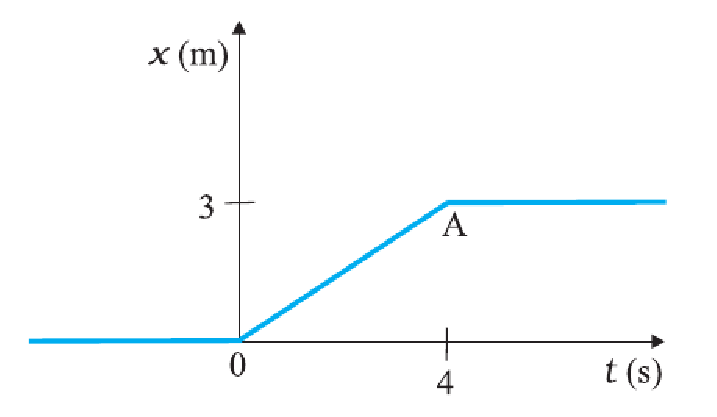
\includegraphics[width=\columnwidth]{./figs/11-1/5/5.16.eps}
\caption{}
\label{fig:5.16}
\end{figure}
\item  A body of mass 0.5 kg travels in a straight line with velocity $v =a x^{\frac{3}{2}}$ where $a = 5 m^{–1/2}s^{-1}$ .
What is the work done by the net force during its displacement from x = 0 to x = 2 m ?
\end{enumerate}
